\section{Auswertung}
Im Folgenden wird zunächst die Spin-Gitter-Relaxationszeit $T_1$
und Spin-Spin-Relaxationszeit $T_2$ bestimmt. Mit diesen Ergebnissen erfolgt anschließend die Bestimmung
der Diffusionskonstante von Wasser. Aufgrund der vielen Messwerte sind die entsprechenden 
Messwerttabellen im Anhang aufgeführt und werden in den jeweiligen Auswertungsteilen referenziert. 
Die Auswertung erfolgt mit der Programmiersprache \textit{Python} und den Paketen \textit{SciPy} \cite{SciPy} und
\textit{NumPy} \cite{NumPy}. Für die Datenvisualisierung wird das Paket \textit{Matplotlib} \cite{Matplotlib} 
verwendet, die Fehlerrechnung wird mit dem Paket \textit{uncertainties} \cite{uncertainties} automatisiert.

\subsection*{Bestimmung der Spin-Gitter-Relaxationszeit}
Zur Bestimmung der Spin-Gitter-Relaxationszeit $T_1$ wird für die genommen Messwerte, aufgeführt in Tabelle 
\ref{tab:T_1}, eine Ausgleichsrechnung mit der Funktion 
\begin{equation*}
    U(t) = M_0 \cdot \left(1 - 2 e^{-\frac{t}{T_1}}\right) 
\end{equation*}
durchgeführt \cite{Finke}. Die Messwerte und die Ausgleichskurve sind in Abbildung \ref{fig:T_1} dargestellt.
\begin{figure}
    \centering
    \includegraphics[width=0.9\linewidth]{figures/T_1.pdf}
    \caption{Gemessene Spannungsamplituden $U$, aufgetragen gegen die Pulsabstände $\tau$. Ebenfalls dargestellt
            ist die berechnete Ausgleichskurve. Die $x$-Achse ist logarithmiert.}
    \label{fig:T_1}
\end{figure}
Aus der Ausgleichsrechnung ergeben sich die Parameter
\begin{align*}
    M_0 &= \SI{1.154(31)}{\volt} \\
    T_1 &= \SI{2.39(8)}{\second} \, .
\end{align*}

\subsection*{Bestimmung der Spin-Spin-Relaxationszeit}
Die Bestimmung der Spin-Spin-Relaxationszeit $T_2$ erfolgt mit dem Meiboom-Gill-Verfahren. Die 
mit dem Oszilloskop aufgenommenen Messwerte sind in Tabelle \ref{tab:T_2} aufgeführt und in Abbildung
\ref{fig:T_2} dargestellt. Verwendet werden immer nur die Spannungsamplituden zu geradzahligem Vielfachen
von $2 \tau$. Zu diesen Echomaxima wird eine Ausgleichsrechnung mit 
\begin{equation*}
    U(t) = M_0 \cdot e^{-\frac{t}{T_2}} + M_1
\end{equation*}
durchgeführt. Die Ausgleichsparameter sind
\begin{align}
    M_0 &= \SI{0.975(14)}{\volt} \\
    M_1 &= \SI{-0.008(16)}{\volt} \\
    T_2 &= \SI{1.37(7)}{\second} \, .
    \label{eq:T_2}
\end{align}
\begin{figure}
    \centering
    \includegraphics[width=0.9\linewidth]{figures/T_2.pdf}
    \caption{Gemessene Spannungsamplituden $U$, aufgetragen gegen die Pulsabstände $\tau$. Verwendet wird die 
            Meiboom-Gill-Methode, sodass nur die Spannungsamplituden zu geradzahligem Vielfachen
            von $2 \tau$ dargestellt sind und in der Ausgleichsrechnung berücksichtig werden. Ebenfalls dargestellt
            ist die berechnete Ausgleichskurve.}
    \label{fig:T_2}
\end{figure}
In Abbildung \ref{fig:Carr_Purcell} ist außerdem der mit dem Oszilloskop aufgenommene zeitliche Verlauf der 
Spannungsamplituden $U$ für die Carr-Purcell-Methode dargestellt, wobei der Pulsabstand $\tau = 22 \text{ ms}$
beträgt.
\begin{figure}
    \centering
    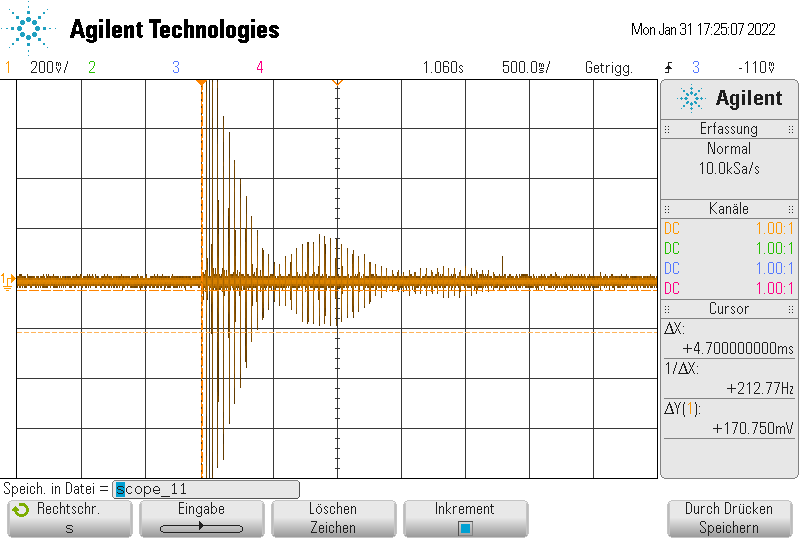
\includegraphics[width=0.9\linewidth]{Messwerte/Carr_Purcell.png}
    \caption{Oszilloskopbild des zeitlichen Verlaufs der Spannungsamplituden $U$ bei Verwendung der 
            Carr-Purcell-Methode. Der Pulsabstand ist $\tau = 22 \text{ ms}.$}
    \label{fig:Carr_Purcell}
\end{figure}

\subsection*{Bestimmung der Diffusionskonstante}
Um die Diffusionskonstante aus den Spannungsamplituden
ermitteln zu können, muss die Diffusionszeit $T_D$ und die Gradientenstärke $g$ bekannt sein.
Zur Bestimmung der Diffusionszeit wird für die Messwerte, aufgeführt in Tabelle \ref{tab:diffusionszeit},
eine Ausgleichsrechnung mit der Funktion
\begin{equation*}
    U(t) = M_0 e^{-\frac{2t}{T_2}} e^{-\frac{t^3}{T_D^*}} + M_1
\end{equation*}
durchgeführt, wobei für $T_2$ der im vorherigen Auswertungsteil bestimmte Wert \ref{eq:T_2}
verwendet wird und $T_D^*$ den Fitparameter kennzeichnet.
Die Messwerte sowie die berechnete Ausgleichskurve sind in Abbildung \ref{fig:echo} dargestellt.
Zur besseren Übersicht über die Messwerte und die Ausgleichskurve ist der Verlauf sowohl als 
linearer Plot (unten), als auch mit logarithmierter $x$-Achse (oben) dargestellt.
\begin{figure}
    \centering
    \includegraphics[width=0.9\linewidth]{figures/echo.pdf}
    \caption{Darstellung der Spannungsamplituden in Abhängigkeit der Pulsabstände. Aufgetragen ist die 
    Funktion $\ln (U(\tau)) - 2 \frac{\tau}{T_2}$ gegen $\tau^3$.
    Zur besseren Übersicht über die Messwerte und die Ausgleichskurve ist der Verlauf sowohl als 
    linearer Plot (unten), als auch mit logarithmierter $x$-Achse (oben) dargestellt.}
    \label{fig:echo}
\end{figure}
Aus der Ausgleichsrechnung ergeben sich die Parameter
\begin{align*}
    M_0 &= \SI{1.201(12)}{\volt} \\
    M_1 &= \SI{0.075(12)}{\volt} \\
    T_D &= \SI{1.64(4)e-6}{\second} \, .
\end{align*}

Die Gradientenstärke kann mit einer Fouriertransformation
des Spektrums des Otto-Hahn-Verfahrens ermittelt werden. 
Dazu werden die mit dem Oszilloskop aufgenommenen Messdaten modifziert indem eine Phasenkorrektur durchgeführt wird und das Signal so 
abgeschnitten wird, dass es genau beim Maximum des Realteils beginnt. Außerdem wird die Amplitude des ersten
Messpunktes halbiert.
In Abbildung \ref{fig:fourier_plot} ist der zeitliche Verlauf des Real- und Imaginärteils der gemessenen 
Spannungsamplituden vor der Modifikation der Messdaten (oben) und danach (unten) dargestellt. 
Der Pulsabstand ist $\tau = 0.2 \text{ ms}$. Die gestrichelte vertikale Linie kennzeichnet den Punkt, bis zu 
dem die Messdaten abgeschnitten werden.
\begin{figure}
    \centering
    \includegraphics[width=0.9\linewidth]{figures/fourier_plot.pdf}
    \caption{Zeitlicher Verlauf des Real- und Imaginärteils der gemessenen 
    Spannungsamplituden vor der Modifikation der Messdaten (oben) und danach (unten) dargestellt. 
    Der Pulsabstand ist $\tau = 0.2 \text{ ms}$. Die gestrichelte vertikale Linie kennzeichnet den Punkt, bis zu 
    dem die Messdaten abgeschnitten werden.}
    \label{fig:fourier_plot}
\end{figure}
Das Fourier-transformierte Spektrum ist in Abbildung \ref{fig:fourier_trafo} dargestellt. Der Abstand $d_f$ der 
beiden Punkte, die sich bei möglichst niedrigen Beträgen der Frequenz $f$ im positiven und negativen Bereich
sehr nah an der $x$-Achse befinden (gekennzeichnet durch die gestrichelte Linie), ist
\begin{equation*}
    d_f = 15,44 \, \text{kHz} \, .
\end{equation*}
\begin{figure}
    \centering
    \includegraphics[width=0.9\linewidth]{figures/fourier_trafo.pdf}
    \caption{Fouriertransformierte des Spektrums zur Bestimmung der Gradientenfeldstärke.
    Der Abstand $d_f$ ist gekennzeichnet durch die gestrichelte Linie (siehe Text).}
    \label{fig:fourier_trafo}
\end{figure}
Die Gradientenstärke berechnet sich nach
\begin{equation*}
    g = \frac{2 \pi d_f}{\gamma d} \, ,
\end{equation*}
wobei $\gamma = 267,52 \, \frac{1}{\text{sT}}$ das gyromagnetische Verhältnis \cite{SciPy} und
$d = 4,2 \, \text{mm}$ der Probendurchmesser ist,
zu 
\begin{equation*}
    g = 0,0864 \, \frac{\text{T}}{\text{m}} \, .
\end{equation*}

Mit der Gradientenstärke und Diffusionszeit kann nun die Diffusionskonstante $D$ bestimmt werden. 
Diese berechnet sich durch Umstellen von Formel \ref{eq:diffusionskonstante}. Aufgrund der Ausgleichsrechnung 
muss diese Formel modifiziert werden zu 
\begin{equation*}
    D = \frac{3}{2} \frac{1}{\gamma^2 G^2 T_D^*} \, .
\end{equation*}
Die Diffusionskonstante ist dann 
\begin{equation*}
    D = (1,71 \pm 0,04) \cdot 10^{-9} \, \frac{\text{m}^2}{\text{s}} \, .
\end{equation*}
